% SARA -- IEEE conference paper (IEEEtran, conference mode).
% Every number is taken from the thesis results chapter; see ../../02_RESULTS_MASTER_TABLE.md for the source of each.
% Compile: pdflatex main ; bibtex main ; pdflatex main ; pdflatex main
\documentclass[conference]{IEEEtran}
\IEEEoverridecommandlockouts
\usepackage{cite}
\usepackage{amsmath,amssymb}
\usepackage{graphicx}
\usepackage{booktabs}
\usepackage{multirow}
\usepackage{xcolor}
\usepackage{tikz}
\usetikzlibrary{positioning,arrows.meta}
\usepackage[hidelinks]{hyperref}
\usepackage{adjustbox}
\graphicspath{{figures/}}
\def\UrlBreaks{\do\/\do-\do\_}
\newcommand{\pp}{\,pp}

\begin{document}

\title{SARA: An Offline Bangla Assistive Smart Glass with Never-Accusing Banknote Screening on a Raspberry~Pi~5}

% TODO: add e-mail addresses and ORCIDs; mark the corresponding author.
\author{\IEEEauthorblockN{MD Abdun Fattah Lam, Mukut Protim Memo, Tanjila Hossain Tapti, Mohammad Shidujaman}
\IEEEauthorblockA{Department of Computer Science and Engineering, Independent University, Bangladesh, Dhaka, Bangladesh}}

\maketitle

\begin{abstract}
Blind people in Bangladesh still depend on others to tell them which banknote they hold, whether it is real, and what a label says. We present SARA, a wearable smart glass that runs entirely on a Raspberry~Pi~5, speaks Bangla, reads Bangla and English, names objects and recognises Bangladeshi Taka notes. Three findings come out of building its currency path. First, a Taka detector trained only on 22,333 automatically labelled composites names 91.5\% of 1,536 independent photographs correctly, and synthetic hand-held close-ups raise its accuracy on real hand-held notes from 11.8\% to 47.5\%. Second, a multi-view counterfeit model trained with all six views of a note collapses to 71.2\% when it sees one view; training on random view prefixes keeps it at 98.2\% (three seeds). Third, the standard split of the JaalTaka dataset tests known reprints: 279 of 322 readable 500~Taka counterfeits share one serial number, and a serial lookup alone scores 90.2\%. On a print-disjoint split, accuracy falls by about eight points, and a watermark check restores it to 95.0\%. Because a wrong verdict harms a blind user, the glass never says ``counterfeit''; it says ``likely genuine'' only above the highest score of any validation counterfeit, a rule with a distribution-free bound of $1/(n{+}1)$. No test counterfeit was passed (0 of 88). On the Pi, a currency answer takes 327\,ms. We report the limits as plainly as the gains: no test through the glass camera and no completed user study yet.
\end{abstract}

\begin{IEEEkeywords}
assistive technology, smart glass, visually impaired, Bangla OCR, banknote recognition, counterfeit detection, multi-view learning, selective prediction, edge AI, Raspberry Pi
\end{IEEEkeywords}

\section{Introduction}
At least 2.2 billion people live with a near or distance vision impairment, and its prevalence in low- and middle-income regions is about four times that in high-income regions \cite{who2023vision}. For a blind person in Bangladesh, three everyday questions usually need another person: which Taka note was handed back and whether it is real, what a medicine label or sign says, and what is ahead. Commercial reading glasses such as OrCam MyEye \cite{orcam} do not list Bangla among their languages or recognise Taka notes, and research glasses often send each picture to a server \cite{googleglass2021,airis2024}. Work on Bangladeshi counterfeits \cite{uddin2016counterfeit,pathak2024counterfeit,chowdhury2022uvink} has not been built into a wearable.

SARA (Smart Assistive Reading Aid) answers these questions on the glass itself. Its currency path also raised questions that matter beyond this device: how to train a detector without hand labels, how a multi-view model behaves when a user captures fewer views, whether a counterfeit benchmark measures what it seems to, and how to give advice that never wrongly accuses a note. Our contributions are:
\begin{itemize}
\item A complete five-mode Bangla assistive glass on a Raspberry~Pi~5, with accuracy reported per module and latency measured on the device.
\item Zero-annotation Taka detection from composites, and synthetic hand-held close-ups that roughly quadruple accuracy on real hand-held notes.
\item The \emph{view-count collapse} of jointly trained multi-view fusion networks, its cause, and a one-line fix (prefix sampling), shown in a controlled comparison.
\item A serial-number audit that exposes a shortcut in the standard JaalTaka split \cite{jaaltaka}, and a print-disjoint split on which a watermark check, including a 47,818-parameter physics-based checker (DMWR), recovers most of the loss.
\item A never-accusing verdict policy with a conformal bound, evaluated on close-up and whole-note photographs.
\end{itemize}

\section{Related Work}
\textbf{Assistive glasses.} OrCam MyEye reads printed text and some banknotes offline, but Bangla is not among the languages it lists \cite{orcam}. Glass-based scene analysis \cite{googleglass2021} and AIris \cite{airis2024} rely on a server, and Raspberry~Pi reading aids are mostly English-only \cite{readingaid_rpi2023}.
\textbf{Taka recognition and counterfeits.} NSTU-BDTAKA trained a YOLOv5 detector on 3,111 annotated images \cite{nstubdtaka2024}. Uddin et al.\ classified watermark, micro-printing and hologram features with an SVM \cite{uddin2016counterfeit}; Pathak et al.\ trained CNNs on note photographs \cite{pathak2024counterfeit}; Chowdhury et al.\ detected the UV flecks of Taka notes with a region proposal network (96.3\%) \cite{chowdhury2022uvink}. JaalTaka provides six close-up views of 1,390 genuine and seized counterfeit notes \cite{jaaltaka,piyas2026jaaltaka}.
\textbf{Methods.} We build on copy-paste augmentation \cite{copypaste2021,tobin2017domain}, multi-view fusion \cite{mvcnn} and modality dropout \cite{moddrop}, selective prediction \cite{chow1970,selective2017} and conformal prediction \cite{vovk2005}. Our split audit follows the literature on shortcuts and leakage \cite{geirhos2020shortcut,kapoor2023leakage}.

\section{The SARA Glass}
\textbf{Hardware.} A Raspberry~Pi~5 (8\,GB) sits in a ventilated rear enclosure. The front of a 3D-printed frame carries a USB webcam (Logitech C270, 640$\times$480; a Camera Module~2 on the first prototype) and a small UV-A lamp (360--395\,nm), and the temple carries five buttons. Feedback comes through a bone-conduction headphone and a vibration motor (Fig.~\ref{fig:proto}).

\begin{figure}[t]
\centering
\includegraphics[width=0.62\columnwidth]{sara_v2_collage.jpg}
\caption{Second SARA prototype: camera and UV lamp at the front, five buttons and a bone-conduction headphone at the side, and the Raspberry~Pi~5 in a ventilated rear enclosure.}
\label{fig:proto}
\end{figure}

\textbf{Modes.} Five modes are available (Fig.~\ref{fig:arch}): Bangla/English text reading (CRAFT \cite{craft} + EasyOCR \cite{easyocr}); object announcement (YOLOv8s \cite{ultralytics}, COCO \cite{coco}); Taka recognition with a safe counterfeit check; facial expression (EfficientNet-V2-S \cite{efficientnetv2}, RAF-DB \cite{rafdb}); and an optional online scene description, the only mode that needs the internet. Modes are started with a button or a voice command that begins with the wake word ``glass'' (Vosk \cite{vosk}). Answers are spoken with Piper \cite{piper}, with espeak-ng \cite{espeakng} as a fall-back. A thermal governor slows background object scans when the board is hot; button presses are never delayed.

\begin{figure}[t]
\centering
\resizebox{\columnwidth}{!}{%
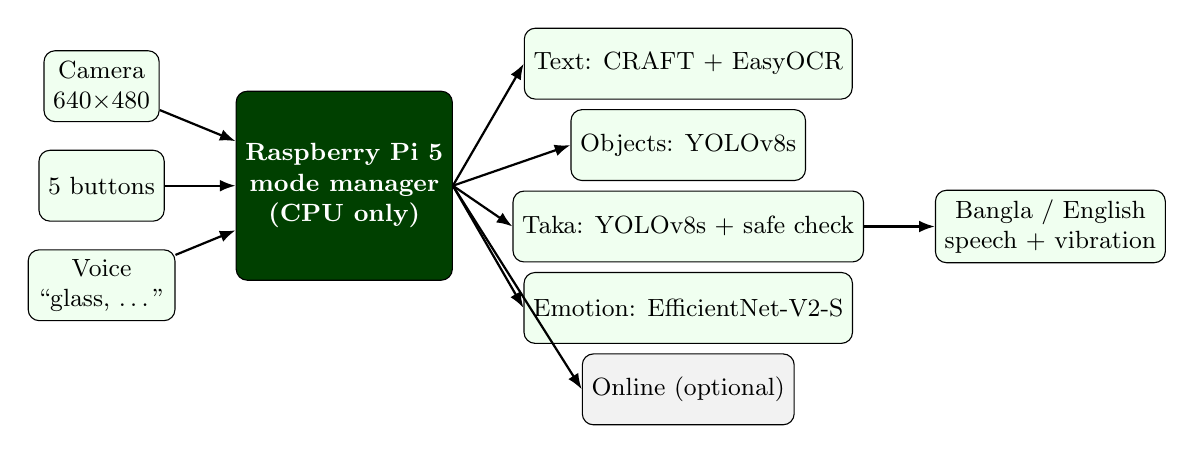
\begin{tikzpicture}[font=\small, node distance=0.35cm and 0.55cm,
  box/.style={draw, rounded corners, align=center, minimum height=0.9cm, fill=green!6},
  pi/.style={draw, rounded corners, align=center, minimum height=2.4cm, fill=green!25!black, text=white, font=\small\bfseries},
  arr/.style={-{Latex[length=2mm]}, thick}]
\node[box] (cam) {Camera\\640$\times$480};
\node[box, below=of cam] (btn) {5 buttons};
\node[box, below=of btn] (mic) {Voice\\``glass, \dots''};
\node[pi, right=0.9cm of btn] (pi) {Raspberry Pi 5\\mode manager\\(CPU only)};
\node[box, right=0.9cm of pi, yshift=1.55cm] (t) {Text: CRAFT + EasyOCR};
\node[box, below=0.12cm of t] (o) {Objects: YOLOv8s};
\node[box, below=0.12cm of o] (c) {Taka: YOLOv8s + safe check};
\node[box, below=0.12cm of c] (e) {Emotion: EfficientNet-V2-S};
\node[box, below=0.12cm of e, fill=gray!10] (n) {Online (optional)};
\node[box, right=0.9cm of c] (sp) {Bangla / English\\speech + vibration};
\foreach \s in {cam,btn,mic} \draw[arr] (\s) -- (pi);
\foreach \m in {t,o,c,e,n} \draw[arr] (pi.east) -- (\m.west);
\draw[arr] (c.east) -- (sp);
\end{tikzpicture}}
\caption{SARA pipeline. All modes except the online description run on the Pi's CPU.}
\label{fig:arch}
\end{figure}

\section{Methods}
\subsection{Taka detection without hand labels}
We pasted 5,073 background-free note images of all nine denominations \cite{banglataka} onto random crops of COCO photographs \cite{coco}, applying perspective tilt, rotation ($\pm30^\circ$), scaling (25--90\% of the frame), colour jitter, motion blur, noise and JPEG compression. The box label follows directly from the paste geometry, so the 22,333 pictures (17,839 / 2,212 / 2,282 for training, validation and test, split by physical note) required no annotation. A YOLOv8s detector was trained for 80 epochs without flips, since a mirrored note is not a real note. For notes held in the hand, we generated 6,000 synthetic close-ups from training notes only, showing notes that fill or overflow the frame, are folded, turned or blurred, or are crossed by finger shapes, and we fine-tuned the detector on them. The epoch and the announce threshold were fixed on 1,611 NSTU validation photographs before any test photograph was read.

\subsection{Prefix training against view-count collapse}
JaalTaka photographs each note in six ordered views. A fusion network trained always with six views is never shown what to do with one, so its one-view behaviour depends on the random initialisation. \emph{Prefix training} keeps a random prefix of $k\sim\mathcal{U}\{1,\dots,6\}$ views per training note. To isolate the cause, we trained the same network four ways (fixed or prefix sampling, crossed with shared or per-view-count batch normalisation) on three seeds each.

\subsection{Serial audit and a print-disjoint split}
A genuine note has a unique serial number, whereas every copy of a counterfeit print carries the same one. We read the serials of the JaalTaka notes by OCR. Of the 322 readable 500~Taka counterfeits, 279 carry one serial, while genuine notes have almost one serial each. On the usual note-disjoint test split, 68 of 87 counterfeits share a serial with a training counterfeit, and the rule ``counterfeit if the serial was seen among training counterfeits'' scores 90.2\%, a shortcut \cite{geirhos2020shortcut}. We therefore built a print-disjoint split (946 / 222 / 222 notes) whose test set has 121 genuine and 101 counterfeit notes from about 24 prints never seen in training.

\subsection{Watermark check and DMWR}
A back-lit note gives $I\approx L\,t$, the lamp $L$ times the paper transmittance $t$, in which the watermark lives. A learned MobileNetV3-Small localizer \cite{mobilenetv3} finds the watermark window, and a MobileNetV2 \cite{mobilenetv2} classifies it. The \emph{denomination-matched watermark residual} (DMWR) works from this physics directly. It first removes the lamp, $Q=\mathrm{z}\big(I/(G_{16}*I)\big)$, where $\mathrm{z}(\cdot)$ standardises to zero mean and unit variance. It then builds a genuine portrait of each note value, $T_d=\mathrm{median}_{n\in\mathcal{G}_d}Q_n$, from genuine training notes only, and forms the residual $R=Q-T_d$. Two small convolutional streams read $Q$ and $R$, and four summary numbers are added: $\rho(Q,T_d)$, $\mathrm{std}(R)$, $\mathrm{Var}(\nabla^2R)$ and the fine-detail energy of $Q$. The whole classifier has 47,818 parameters (0.21\,MB). In the hybrid, the network and watermark log-odds are combined by a logistic regression fitted on validation notes.

\subsection{A verdict that never accuses}
On the glass, four windows are cut from the detected note at the positions of JaalTaka views 1--4, and the authenticator returns $p$. The glass says ``likely genuine'' if $p>\tau$, and otherwise ``check by hand whether it is genuine''. It never says ``counterfeit''. The threshold $\tau=0.99959$ is the highest score of any of the $n=88$ validation counterfeits. For a new counterfeit exchangeable with them, $P(p_{\text{new}}>\tau)=1/(n+1)=1.1\%$ \cite{vovk2005}. An image-quality gate rejects dark and blurred frames first.

\section{Results}
All choices were made on validation data, each test set was read once, and trained models were repeated with seeds 42--44. Laptop numbers come from an RTX~3050 laptop GPU; device numbers come from a Raspberry~Pi~5 (8\,GB).

\textbf{Taka detection} (Table~\ref{tab:det}). The detector is almost perfect on held-out composites. On independent photographs it names 91.5\% of notes correctly, and the hand-held fine-tune lifts hand-held accuracy from 11.8\% to 47.5\% on the laptop and from 8.7\% to 33.5\% on the Pi (INT8). The fine-tune has costs: unknown one-Taka notes are named as a value more often (22.8\% to 36.6\%), and the spoken total of three notes in one picture is right 97.0\% of the time instead of 99.2\%.

\begin{table}[t]
\caption{Taka detection (right note value unless stated)}
\label{tab:det}
\centering\small
\begin{adjustbox}{max width=\columnwidth}\begin{tabular}{@{}lcc@{}}
\toprule
Test set (n) & Earlier & Hand-held FT \\ \midrule
Synthetic composites (2,282), mAP@0.5 & 0.995 & 0.995 \\
Synthetic composites, mAP@0.5:0.95 & 0.849 & 0.848 \\
Bangla Money photos (1,536), laptop & 89.6\% & \textbf{94.1\%} \\
NSTU hand-held (1,127), laptop & 11.8\% & \textbf{47.5\%} \\
NSTU hand-held (1,127), Pi INT8 & 8.7\% & \textbf{33.5\%} \\
One-Taka notes named as a value (101) & 22.8\% & 36.6\% \\ \bottomrule
\end{tabular}\end{adjustbox}\\[2pt]
{\footnotesize The first detector at confidence 0.25 scored 91.5\% on Bangla Money; the earlier column uses the 0.60 announce threshold.}
\end{table}

\textbf{View-count collapse} (Table~\ref{tab:views}, Fig.~\ref{fig:views}). Fixed six-view training reaches 98.1\% with six views but only 71.2\% with one, and its one-view result swings from 131 to 194 correct notes out of 208 across seeds. Prefix sampling alone removes the collapse: 98.2\% at one view with shared batch normalisation (exact McNemar $p\le9.3\times10^{-10}$ on every seed) and no difference at six views ($p\ge0.22$). Frozen ImageNet backbones with a per-view linear probe reach 98--99\% on this split, so we make \emph{no} state-of-the-art claim. Outside currency, prefix training helped an attention-fusion head on MVP-N \cite{mvpn} (40.7\% to 48.0\% at one view) but not a concatenation head, so the benefit depends on the fusion design.

\begin{table}[t]
\caption{Same network, four trainings: accuracy (\%) on 208 JaalTaka test notes, mean $\pm$ sd over 3 seeds}
\label{tab:views}
\centering\small
\setlength{\tabcolsep}{3.5pt}
\begin{adjustbox}{max width=\columnwidth}\begin{tabular}{@{}lcccc@{}}
\toprule
Training & 1 view & 2 views & 4 views & 6 views \\ \midrule
Fixed 6, shared BN & 71.2$\pm$11.4 & 73.1$\pm$17.1 & 90.5$\pm$2.2 & 98.1$\pm$0.5 \\
\textbf{Prefix, shared BN} & \textbf{98.2$\pm$0.7} & \textbf{98.4$\pm$0.3} & \textbf{98.6$\pm$0.5} & \textbf{98.7$\pm$0.3} \\
Fixed 6, per-count BN & 87.2$\pm$9.7 & 92.8$\pm$6.3 & 95.7$\pm$4.6 & 99.0$\pm$0.0 \\
Prefix, per-count BN & 96.5$\pm$1.5 & 98.4$\pm$0.6 & 97.6$\pm$0.8 & 98.1$\pm$1.0 \\ \bottomrule
\end{tabular}\end{adjustbox}
\end{table}

\begin{figure}[t]
\centering
\includegraphics[width=\columnwidth]{fig13_same_arch.png}
\caption{Accuracy against the number of views given at test time for the four trainings (3 seeds, $\pm$1 sd).}
\label{fig:views}
\end{figure}

\textbf{Unseen prints} (Table~\ref{tab:unseen}). On the print-disjoint split, the prefix network falls from about 98\% to 89--90\%. Adding the watermark check gives 94.4\% at one view and 95.0\% at six, the same on every seed. A properly fine-tuned ResNet-50 \cite{resnet} reaches 94.4--94.9\%, so the result is a tie, not a win. A serial blacklist catches none of these counterfeits by construction. With about 24 test prints, the print-level uncertainty is roughly $\pm$12 points, so differences of a few points between methods cannot be established on this dataset.

\begin{table}[t]
\caption{Accuracy on unseen counterfeit prints (222 test notes, 101 counterfeit; mean $\pm$ sd, 3 seeds)}
\label{tab:unseen}
\centering\small
\begin{adjustbox}{max width=\columnwidth}\begin{tabular}{@{}lcc@{}}
\toprule
Checker & 1 view & 6 views \\ \midrule
Frozen ResNet-50 + linear probe & 85.1 & 83.8 \\
Prefix network (ours) & 89.9$\pm$0.7 & 89.3$\pm$1.3 \\
Fine-tuned ResNet-50 (full resolution) & 94.9$\pm$1.8 & 94.4$\pm$2.6 \\
Watermark only (localizer + MobileNetV2) & \multicolumn{2}{c}{92.6$\pm$0.5} \\
\textbf{Prefix network + watermark} & \textbf{94.4$\pm$0.5} & \textbf{95.0$\pm$0.0} \\ \bottomrule
\end{tabular}\end{adjustbox}
\end{table}

\textbf{DMWR.} On the 197 registered print-disjoint test notes, DMWR scores 91.5$\pm$0.3\% (AUC 0.950) against 92.9\% (AUC 0.976) for a fine-tuned MobileNetV2 with 2.23\,M parameters. The difference is not significant (exact McNemar $p=0.375$, 0.688 and 0.375 per seed), while DMWR's model file is about 44 times smaller. Each stream alone reaches 85.8--88.0\% with a 3--5 point spread between seeds, so the portrait and the residual carry complementary information (Fig.~\ref{fig:dmwr}).

\begin{figure}[t]
\centering
\includegraphics[width=\columnwidth]{fig_dmwr_steps.png}
\caption{DMWR on a genuine (top) and a counterfeit (bottom) 500~Taka test note: back-lit window, lamp removed ($Q$), genuine portrait ($T_{500}$), residual ($R$).}
\label{fig:dmwr}
\end{figure}

\textbf{Safety} (Table~\ref{tab:safe}). On whole-note photographs, a plain genuine/counterfeit verdict at $p=0.5$ was wrong on 20--59\% of genuine notes and on 40\% of counterfeits, so it was switched off. The never-accusing policy passed none of the 88 test counterfeits and none of the 20 whole-note counterfeit photographs, and the word ``counterfeit'' was never spoken in 1,889 runs. The price is usefulness: it confirms 57.5\% of genuine close-up notes but few whole notes.

\begin{table}[t]
\caption{Never-accusing verdict policy (Wilson 95\% intervals)}
\label{tab:safe}
\centering\small
\begin{adjustbox}{max width=\columnwidth}\begin{tabular}{@{}lc@{}}
\toprule
Measure & Result \\ \midrule
Counterfeits passed, JaalTaka test & 0 / 88 (0--4.2\%) \\
Counterfeits passed, whole-note photos & 0 / 20 (0--16.1\%) \\
Genuine confirmed, JaalTaka test & 69 / 120 (57.5\%) \\
Genuine confirmed, whole-note photos & 0.4--16.9\% \\
Wrong answers in bad light, with quality gate & 0 / 208 \\ \bottomrule
\end{tabular}\end{adjustbox}
\end{table}

\textbf{Text reading.} On a benchmark with correctly shaped Bangla, selecting the main text block and cleaning the output lowered test CER from 9.3\% to 2.4\%, and for Bangla from 11.9\% to 3.2\%. On 1,000 real word images from ICDAR~2019 MLT \cite{mlt2019}, the error was much higher. A recogniser fine-tuned on real words and blended half-and-half with the released weights lowered it from 39.2\% to 28.7\% for Bangla and from 62.5\% to 50.6\% for Latin script, without losing accuracy on printed text (2.46\% to 2.27\%).

\textbf{Voice commands} (12 held-out synthetic voices, laptop). Commands are carried out 100\% of the time in clean conditions, 98.9\% when whispered, 82.5\% with street noise as loud as the voice, and 54.3\% with people talking nearby at 10\,dB (3.2\% without the wake word). False commands fall from 212 to 13 in 5,040 ordinary sentences.

\textbf{Raspberry~Pi~5.} Median latencies on the first, cool-board run were 327\,ms for the whole currency check, 254\,ms for the INT8 Taka detector, 50\,ms for the watermark check and 37/90\,ms for the authenticator with one or six views. Text reading took about 18.7\,s per capture. Memory peaked at 1.48\,GB over a 30-minute run without throttling. In a second run after two sessions of use, the board reached 88.7\,$^\circ$C and was throttled in 76\% of samples (currency check 399\,ms). A thermal governor was added in response; its effect has not yet been measured. A third run on 29 October, with a fan and a heat sink added and the C270 webcam, read a 3-line sign in 5.4\,s, three times faster than on 1 October, with the currency check at 422\,ms; under 30 minutes of continuous load the processor's sensor reached 87.0\,$^\circ$C with the soft temperature limit active in 55\% of samples. The application's log of that day moved the Pi to the laptop's full-precision Taka detector: 532\,ms a check, and a note named in 5 of 8 presses against 2 of 10 before.

\section{Limitations}
No accuracy figure in this paper was measured through the glass camera. A first informal field test with its 640$\times$480 fixed-focus camera found currency recognition unreliable and Bangla text unread. Trials with a visually impaired participant have started, but no user study is complete and no user result is reported. The unseen-print results rest on about 24 counterfeit prints of one currency, and the whole-note safety evidence on about four physical counterfeits. Voice results use synthetic voices on a laptop. Real-photo OCR remains the weakest mode, and text reading is slow on the Pi.

\section{Conclusion}
SARA shows that a Bangla assistive glass can recognise money, read text and name objects on a Raspberry~Pi~5 without the internet. The currency work also produced lessons that carry beyond this device. Train multi-view models on the view counts users will actually provide. Audit counterfeit benchmarks for repeated prints before trusting their scores. And when the user cannot check the answer, prefer a verdict that never accuses. Code, results and the thesis are public at \url{https://github.com/aflam330/SARA} and \url{https://github.com/aflam330/Senior_project_wearable_glass_for_blind_people_using_ocr_and_ylo}.

\section*{Acknowledgment}
We thank the visually impaired participant who is trying the prototype, and the authors of the JaalTaka, BanglaTaka, NSTU-BDTAKA and Bangla Money datasets for making them public.

\bibliographystyle{IEEEtran}
\bibliography{references_verified}

\end{document}
